\documentclass[11pt,twoside]{report}
\usepackage{preamble}
\graphicspath{{../img/ch6/}}
\setcounter{chapter}{6}

\begin{document}

\chapter{Collective Behaviour of Mutant Fish}
\label{chapter:fish_mutation}

\section{Introduction}

Understanding the behaviours of zebrafish is not only intellectually fulfilling, but it is also useful. Appreciating the stochastic nature of the animal behaviours, the detailed knowledge of zebrafish would enable us identify the behavioural differences among different groups, without being mislead by the randomness of animal behaviours.

Let us take an example from soft matter physics. If I create two canonical ensembles of Lennard--Jones liquid at the same density and temperature (the same $N, V, T$ parameters), and follow the movement of particles, I would get different trajectories, but same thermodynamic quantities, such as the pressure and the entropy, since the systems are equivalent. If these ensembles have different temperature values, I would get wildly different results, even different phases, because the systems are in different states. Nevertheless, I can still confirm these systems are the same if they follow the same equation of states.

I will now extend the argument to the zebrafish. Suppose I have two groups of zebrafish, and they have different statistical quantities, such as the averaged speed and the averaged nearest neighbour (NN) distance, what conclusion should I draw? I have two options. Firstly I can claim these two groups of fish are inherently different, which means they interact with each other in different ways. Alternatively, I can claim that these two groups of fish are in different states, while they have the same intrinsic fish--fish interactions. I can use the equation of states to determine the better conclusion. If the different groups follow the same equation of states, then I am confident that they have the same interaction but were subjection parameters (like LJ system under different temperatures). In another case, I can conclude that the fish are intrinsically different with different fish--fish interactions.

In this chapter, I will use the methods developed before, and study the behavioural change of zebrafish when they were genetically modified. Following a pioneering work \cite{tang2020} that tested the behaviours of different fish groups with different genetic modifications, I will present a more detailed analysis of the behaviours with a specific mutation, for which the \emph{col11a2} gene was changed.

\section{Method}

In this chapter the muatnat fish were placed in my custom 3D tracking system, and their behaviour were analysed using the same tools from chapter \ref{chapter:fish_3d} and \ref{chapter:fish_model}.

We tested two types of 

\section{The Behaviour of col11a2 Mutant Fish}

\subsection{The Behaviour of 1 Mutant Fish}

The col11a2 mutant fish exhibit significant difference comparing with the wt fish.


\begin{SCfigure}
  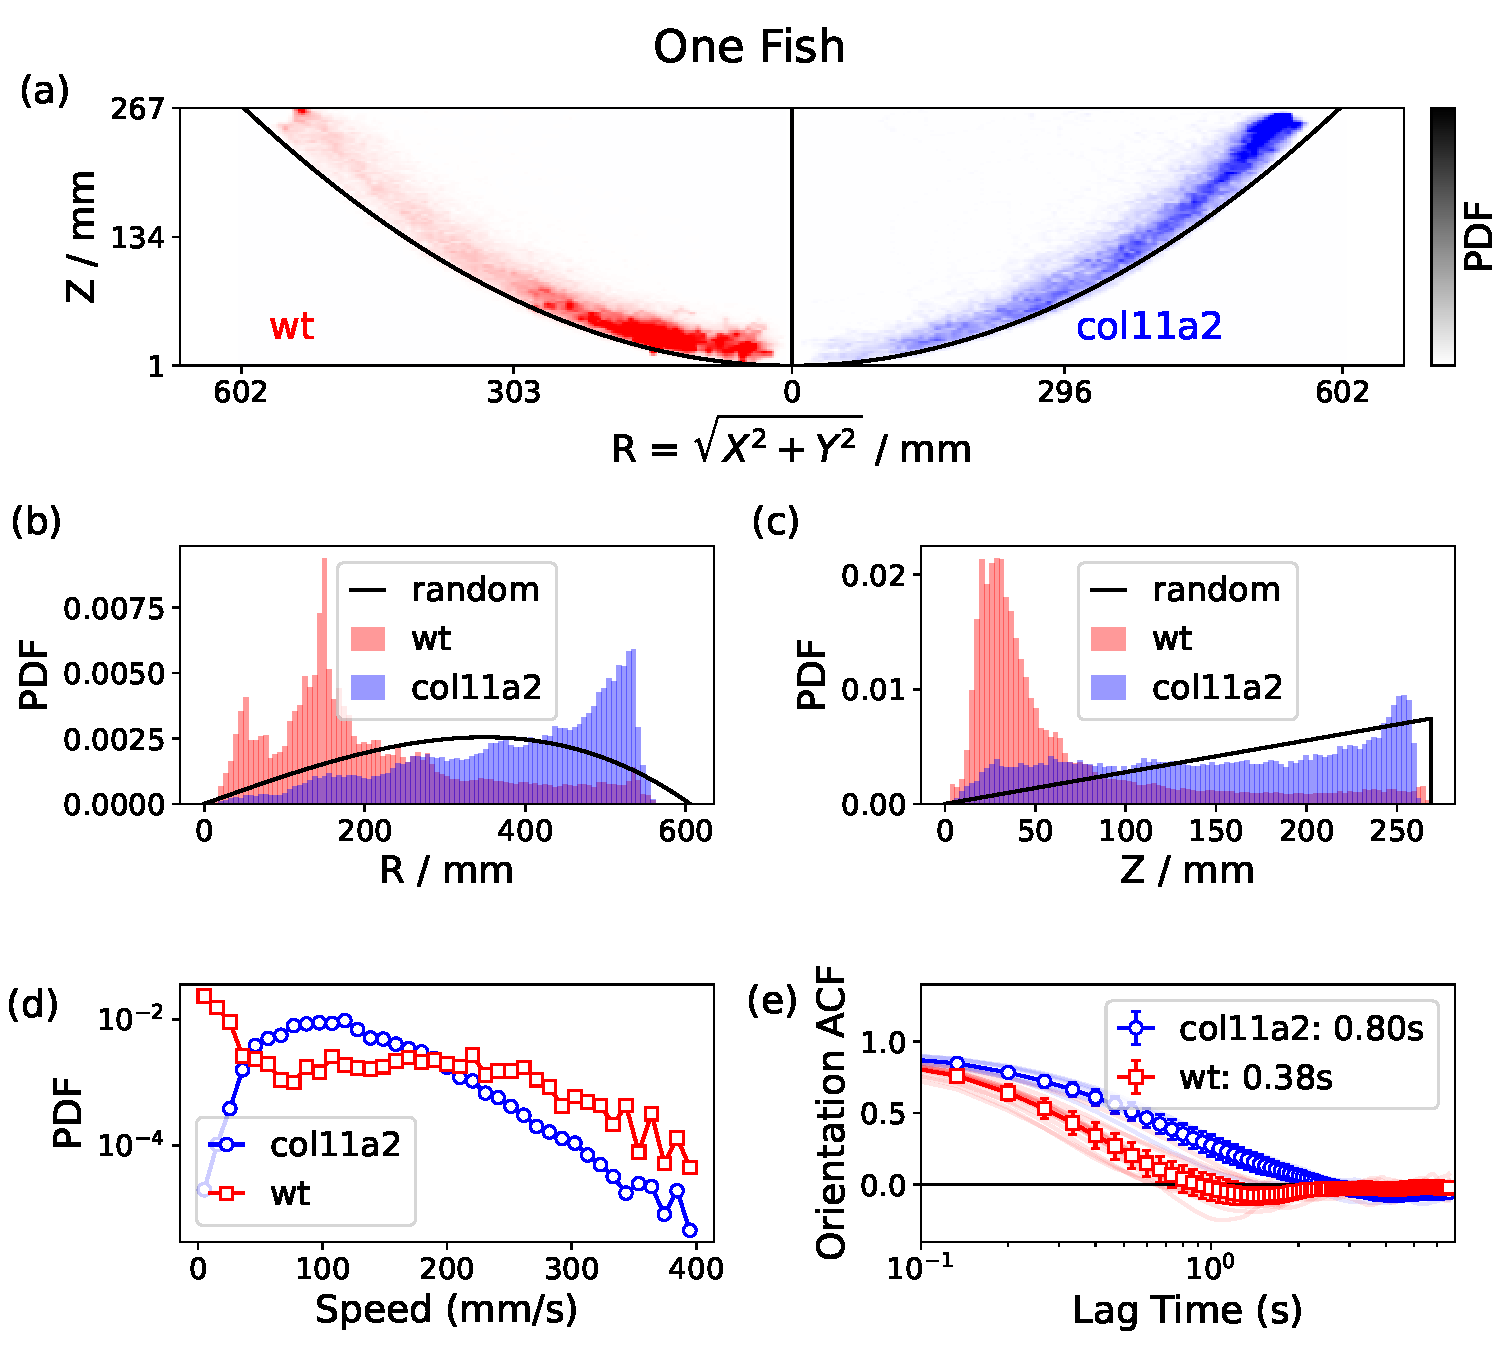
\includegraphics[width=\linewidth]{figOneFish}
  \caption{\label{fig:one_fish_mutant}
  	The bheaviour of 1 mutant fish and 1 wt fish.
  	(a) The joint probability density function (PDF) of the 2D radius and the Z coordinate of the fish.
  	(b) The marginal PDF of the 2D radius. 
  	(c) The PDF of the height of the fish.
  	(d) The distribution of speed of the fish.
  	(e) The average auto-correlation function of the orientation of the fish.
  	The solid line in (a) presents the outline of the observation tank. The solid lines in (b) and (c) indicate the corresponding distributions of ideal gas in the tank.
  }
\end{SCfigure}



\section{The Behaviour of other Mutant Fish} 

\end{document}
